\documentclass[parskip=half,DIV=16]{scrartcl}

\title{Lab assignment 4}
\subtitle{ATM S 544}
\author{Dominik Stiller}
\date{\today}

\usepackage[english]{babel}
\usepackage[utf8]{inputenc}
\usepackage{siunitx,amsmath,physics}
\usepackage{caption,subcaption,graphicx,csquotes,xcolor}
\usepackage{booktabs}
\usepackage{placeins}
\usepackage[
	backend=biber,
	bibwarn=true,
	bibencoding=utf8,
	sortlocale=en_US,
	url=false,
	style=apa,
	isbn=false
]{biblatex}

\definecolor{uw-purple}{RGB}{51, 0, 111}

\usepackage{hyperref}
\hypersetup{
	% hidelinks,
	colorlinks=true,
	linkcolor=black,
	citecolor=black,
	urlcolor=uw-purple
}

\usepackage{doi}
\usepackage{nomencl}
\makenomenclature
\usepackage[noabbrev,capitalise]{cleveref}
\usepackage[acronym,nonumberlist,nopostdot,nogroupskip]{glossaries}
\usepackage[
	outputdir=build,
]{minted}
\setminted{
	linenos,
	tabsize=4,
	fontsize=\small,
}
\newmintinline{python}{}

\usepackage{lmodern}
\usepackage[T1]{fontenc}
\usepackage{inconsolata}
\usepackage{tikz}

\newcommand{\result}[1]{\colorbox{uw-purple}{\textcolor{white}{#1}}}

\setlength{\nomlabelwidth}{1.5cm}
\setlength{\nomitemsep}{-\parsep}
\newcommand{\nomunit}[1]{%
\renewcommand{\nomentryend}{\hspace*{\fill}\si{#1}}}

\sisetup{per-mode=symbol}
\AtBeginDocument{\RenewCommandCopy\qty\SI}

\DeclareGraphicsRule{.ai}{pdf}{.ai}{}

\addbibresource{bibliography.bib}



\begin{document}

\maketitle



\section{Single observation with $N_e = 99$}

\begin{figure}[H]
   \centering
   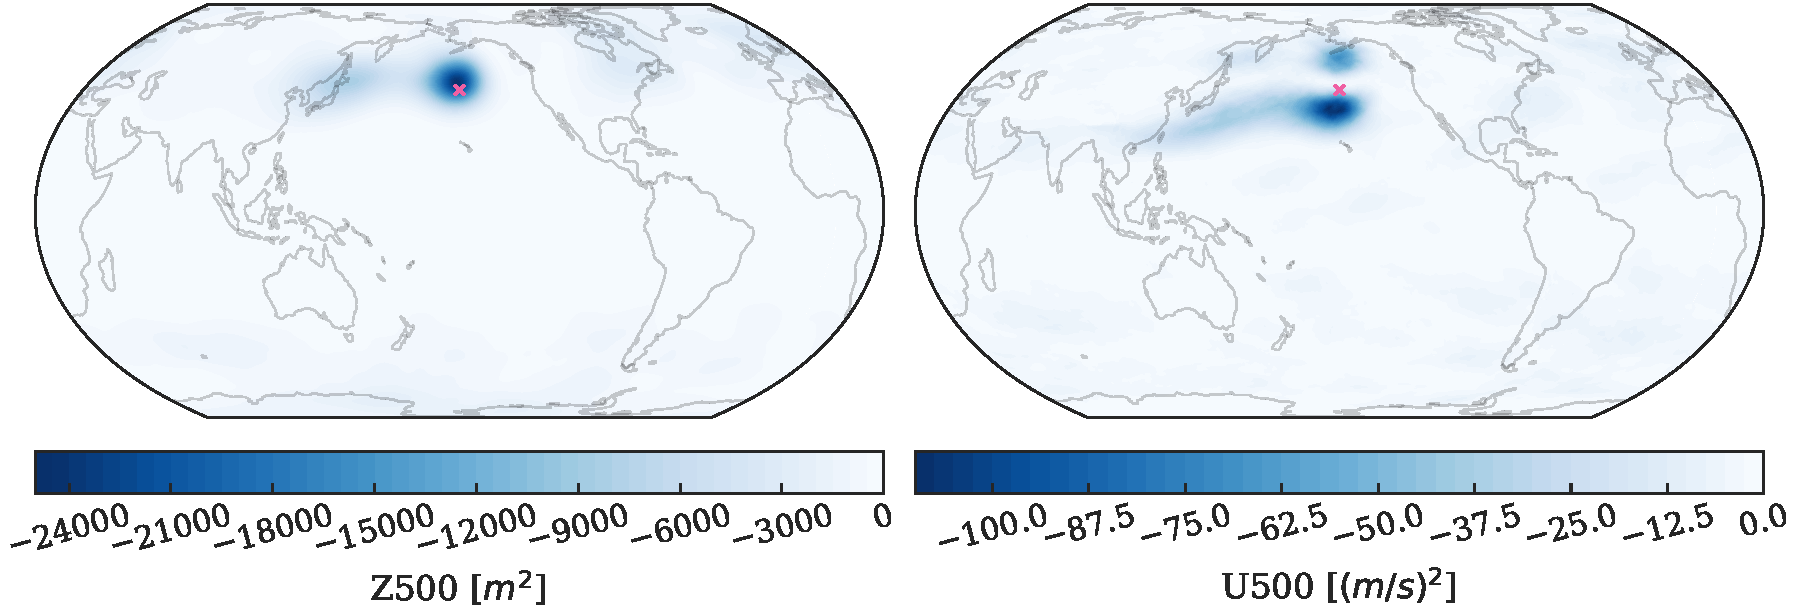
\includegraphics[width=\textwidth]{figures/exp1_prior_post_var.pdf}
   \caption{Difference of case-averaged prior and posterior variances for $N_e = 99$.}
   \label{fig:exp1-1}
\end{figure}

\cref{fig:exp1-1} shows the difference of the case-averaged prior and posterior variances. The Kalman filter update reduces the variance as expected (or rather, required by the equations). The most confidence in the state estimate is gained around the observation location (\textcolor{mpl-pink}{\ding{53}}), particularly for Z500. Zonal winds are affected north and south of the observation location as dictated by geostrophic theory. Moving away from the observation location, the decrease in variance is close to zero.


\begin{figure}[H]
   \centering
   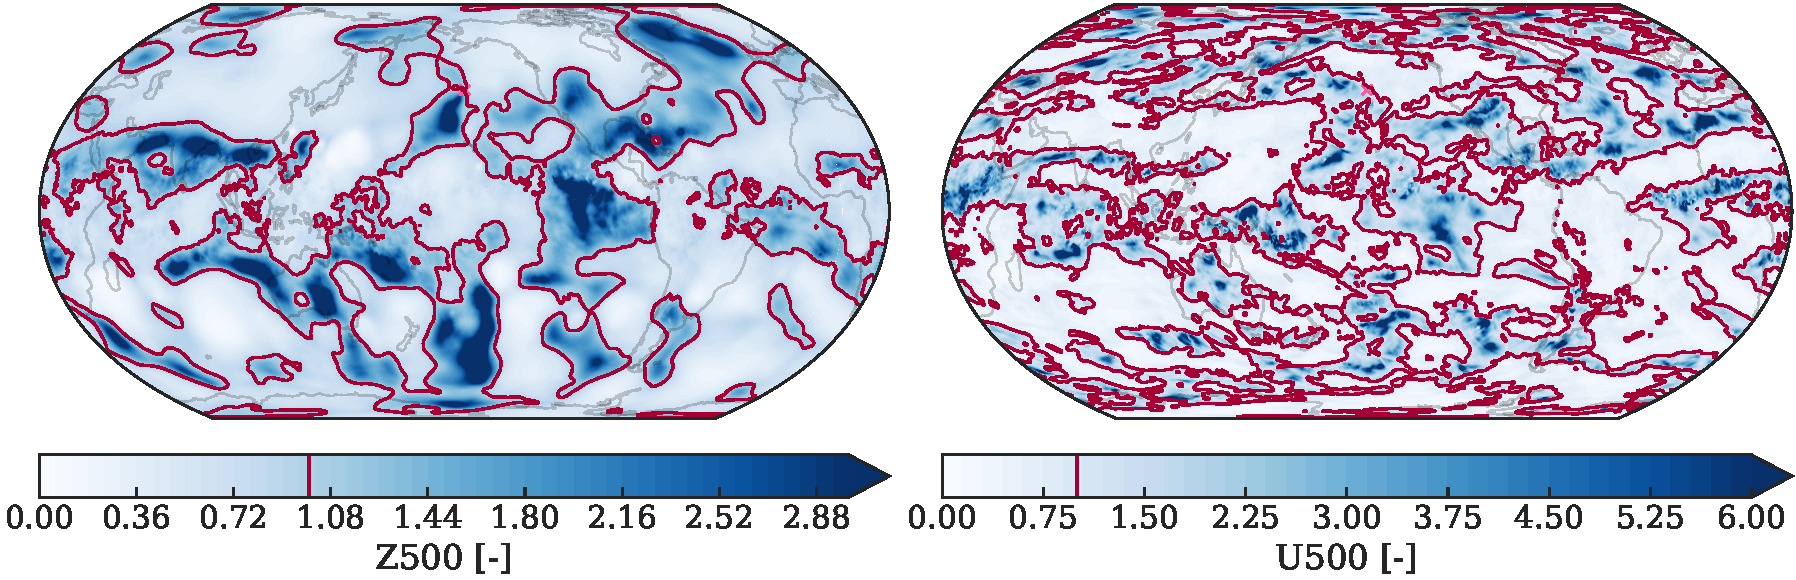
\includegraphics[width=\textwidth]{figures/exp1_var_se_ratio.pdf}
   \caption{Ratio of case-averaged posterior variance and squared error of the posterior mean for $N_e = 99$.}
   \label{fig:exp1-2}
\end{figure}

\cref{fig:exp1-2} shows the ratio of the case-averaged posterior variance to the squared error of the posterior mean. Ideally, their ratio would be 1 (indicated by the red contours) since the variance is a proxy for the squared error. However, the ratio is dominated by the squared error, which is almost exclusively due to the difference of the true global state from climatology (which is the mean state over the 99 members). This is also the case when averaged meriodinally. There is no discernible spatial behavior, not even in the vicinity of the observation.


\begin{figure}[H]
   \centering
   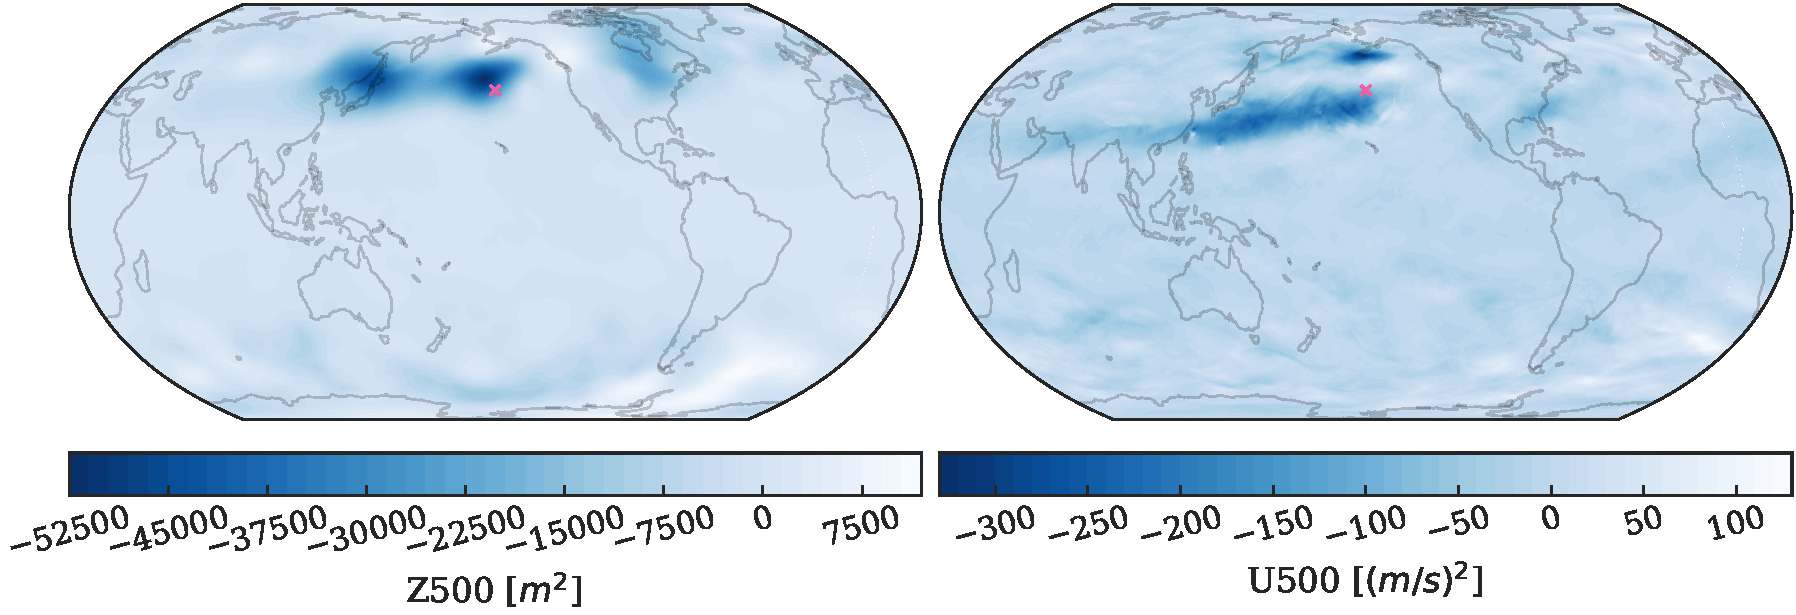
\includegraphics[width=\textwidth]{figures/exp1_prior_post_se.pdf}
   \caption{Difference of case-averaged squared errors of the posterior mean and prior mean for $N_e = 99$.}
   \label{fig:exp1-3}
\end{figure}

\cref{fig:exp1-2} shows the difference of the case-averaged squared errors of the posterior mean and the prior mean. The spatial pattern is similar to the difference in variances from \cref{fig:exp1-1}: large decreases in error around the observations, and generally slightly negative differences. This supports the thesis that the variance is a good proxy for the squared error. Note how some regions show slightly increased errors due to spatial variations in the true state.




\section{Single observation with $N_e = 25$}

\begin{figure}[H]
   \centering
   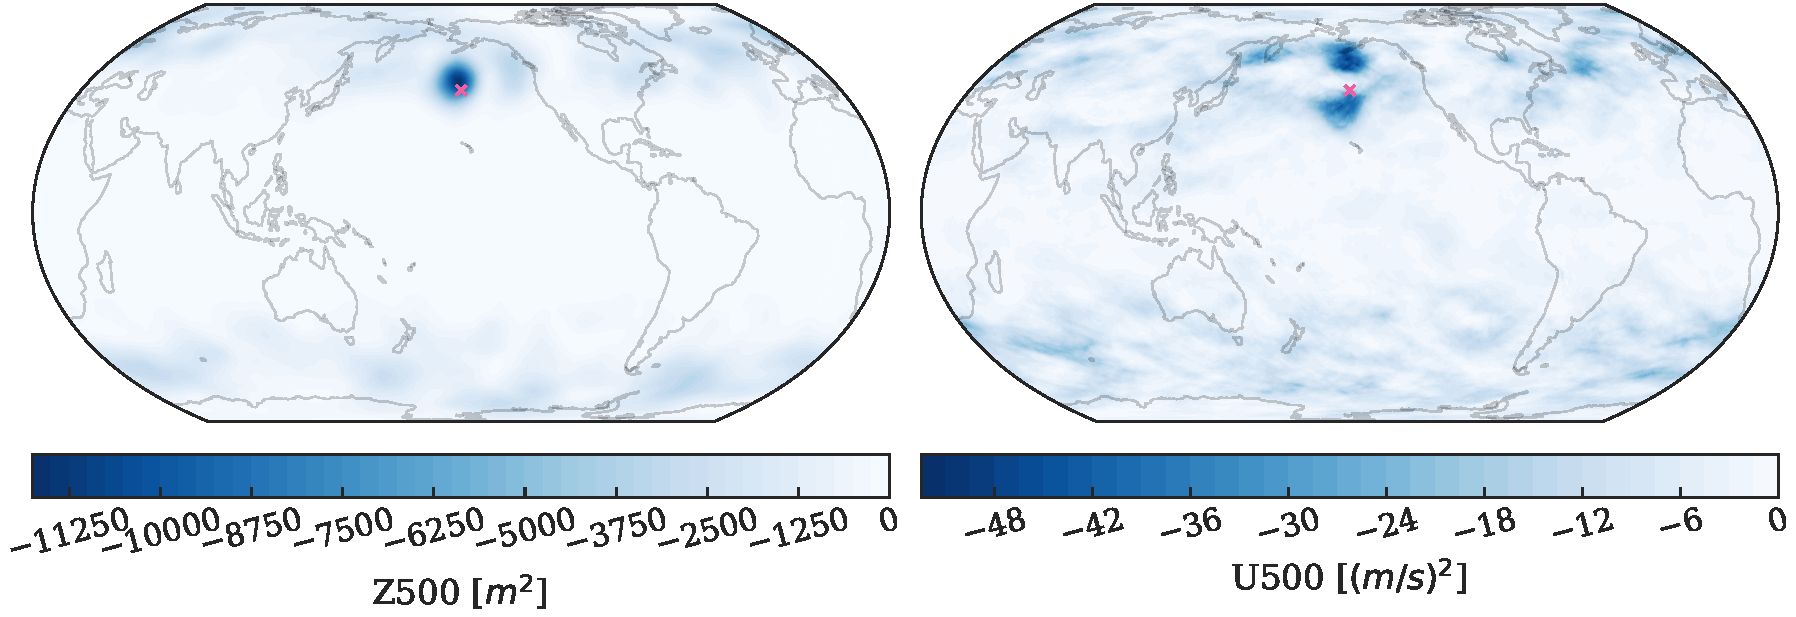
\includegraphics[width=\textwidth]{figures/exp2_prior_post_var.pdf}
   \caption{Difference of case-averaged prior and posterior variance for $N_e = 25$.}
   \label{fig:exp2-1}
\end{figure}

\cref{fig:exp2-1} shows the difference of the case-averaged prior and posterior variances. Since there is less spread to begin with than in the previous experiment (the prior consists of a month's worth of days instead of 3 months), the prior variance is smaller. (About a factor two; is it coincidence that two is the square root of the ratio of ensemble members?) Also, the reduction in variance around the observation location has decreased by a factor two compared to \cref{fig:exp1-1}.

This can be explained as follows. The prior variance (about \qty{20000}{m^2} for $N_e=100$, about \qty{10000}{m^2} for $N_e = 25$) is much larger than the observation variance of \qty{10}{m^2}. Therefore, around the observation location, the posterior mean will essentially be the observation and the posterior variance will be slightly less than \qty{10}{m^2}. This means that the posterior variance at the observation location is independent of $N_e$, which is why the maximum difference is only driven by the prior variance. Away from the observation location, there is no significant difference when changing $N_e$.



% \begin{figure}[h]
%    \centering
%    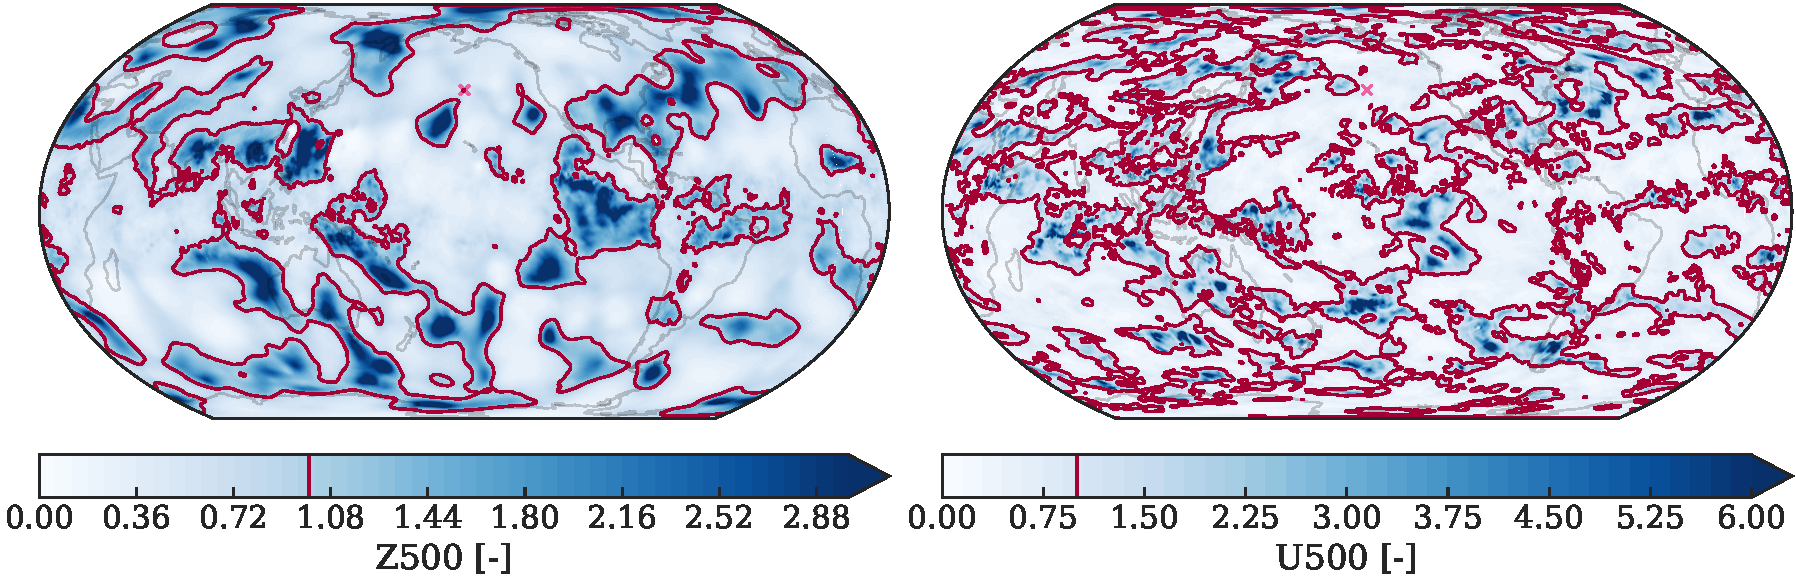
\includegraphics[width=\textwidth]{figures/exp2_var_se_ratio.pdf}
%    \caption{Ratio of case-averaged posterior variance and squared error of the posterior mean for $N_e = 25$.}
%    \label{fig:exp2-2}
% \end{figure}



\begin{figure}[H]
   \centering
   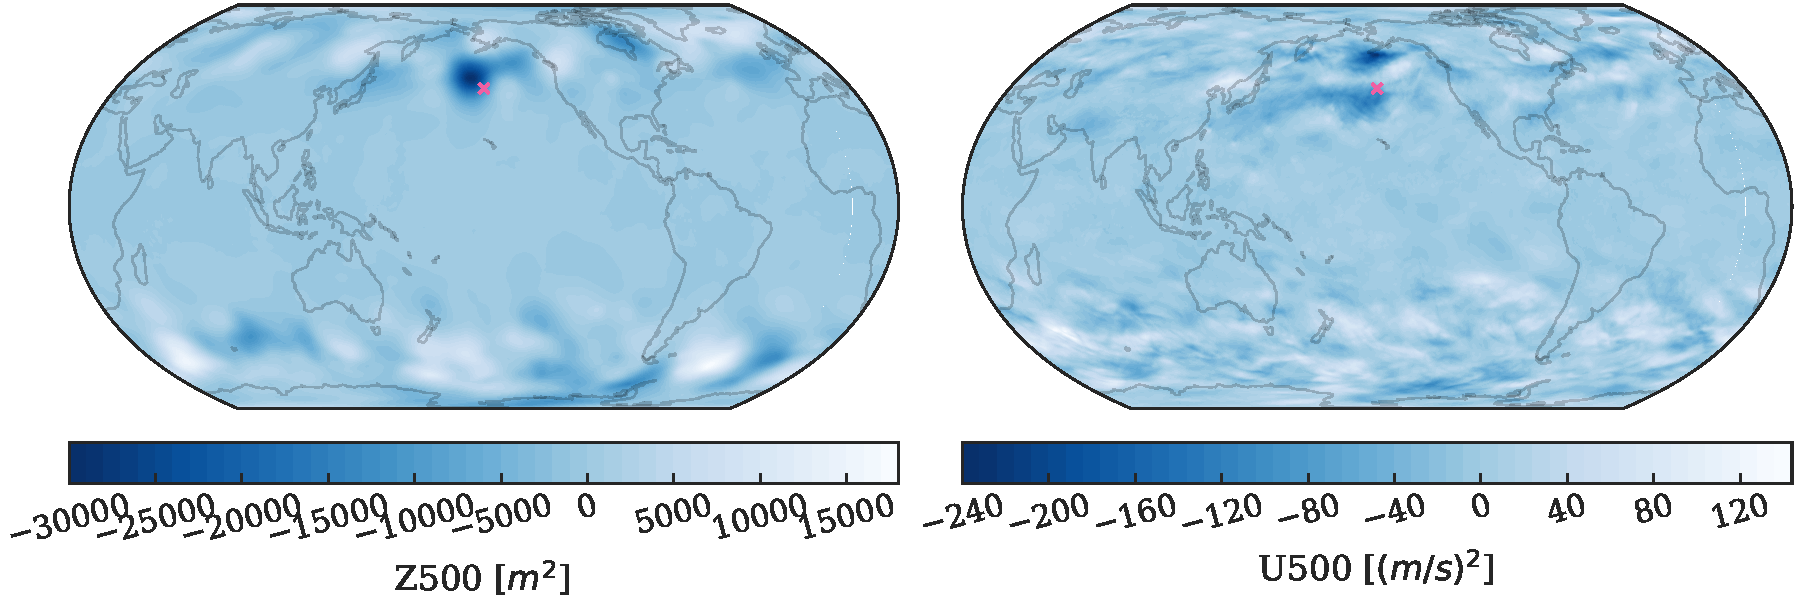
\includegraphics[width=\textwidth]{figures/exp2_prior_post_se.pdf}
   \caption{Difference of case-averaged squared errors of the posterior mean and prior mean for $N_e = 25$.}
   \label{fig:exp2-3}
\end{figure}

\cref{fig:exp2-3} shows the difference of the case-averaged squared errors of the posterior mean and the prior mean. Again, the spatial pattern is correlated with the difference in variances from \cref{fig:exp2-1}, and the squared error is halved similarly.



\end{document}
